\chapter{Approximation Algorithms on Graphs}

The previous chapter left us in an uncomfortable place. Vertex cover, traveling salesman,
max-cut, Steiner tree, set cover --- each is \textsf{NP}-hard, so unless $\textsf{P}=\textsf{NP}$
there is no polynomial-time algorithm that always returns the optimum. But ``no exact algorithm''
is not the same as ``no algorithm.'' For a great many of these problems we can compute, in
polynomial time, a solution provably within a constant factor of optimal. A vertex cover at most
twice the smallest one. A tour at most $3/2$ the shortest one. A cut catching at least $87.8\%$ of
the optimal number of crossing edges. These are \emph{approximation algorithms}, and what makes them
remarkable is that the guarantee is not empirical --- it is a theorem, proved against an optimum we
cannot even compute.

This chapter develops the core toolkit: the combinatorial gems (vertex cover by maximal matching,
Christofides for TSP, the double-tree heuristic for Steiner tree), the LP-relaxation-and-rounding
method (vertex cover again, this time through duality), the greedy method with its $\ln n$ analysis
(set cover), and the semidefinite-programming leap (Goemans--Williamson max-cut). We close with the
deepest story in the chapter: sparsest cut, the $\Oh(\log n)$ Leighton--Rao bound, and the
$\Oh(\sqrt{\log n})$ ARV result --- the gateway to the spectral and electrical-flow material in the
chapters that follow.

\chapterline

\section{What an approximation guarantee means}

\begin{definition}[Approximation ratio]\label{ch38:def-ratio}
Let $\Pi$ be an optimization problem and let $\mathrm{OPT}(I)$ denote the optimal objective value on
instance $I$. A polynomial-time algorithm $\mathcal{A}$ is an \emph{$\alpha$-approximation} if for
every instance $I$ it returns a feasible solution of value $\mathcal{A}(I)$ with
\[
  \frac{\mathcal{A}(I)}{\mathrm{OPT}(I)} \le \alpha \quad\text{(minimization, } \alpha\ge 1\text{)},
  \qquad
  \frac{\mathcal{A}(I)}{\mathrm{OPT}(I)} \ge \alpha \quad\text{(maximization, } \alpha\le 1\text{)}.
\]
We call $\alpha$ the \emph{approximation ratio}. A family of algorithms parameterized by $\eps>0$
giving ratio $1+\eps$ (or $1-\eps$) in time polynomial in the input for each fixed $\eps$ is a
\emph{polynomial-time approximation scheme} (PTAS); if the running time is also polynomial in
$1/\eps$ it is an \emph{FPTAS}.
\end{definition}

\begin{intuitionbox}
The single difficulty is that we must bound our solution against an optimum \emph{we cannot find}. The
trick is always a third quantity --- a \emph{lower bound} $L \le \mathrm{OPT}$ (for minimization) that we
\emph{can} compute, and against which we sandwich our answer:
\[
  L \;\le\; \mathrm{OPT} \;\le\; \mathcal{A}(I) \;\le\; \alpha\cdot L.
\]
If our output is at most $\alpha L$ and $\mathrm{OPT} \ge L$, then $\mathcal{A}(I)\le \alpha\,\mathrm{OPT}$
follows for free. Every algorithm below is, at heart, the art of choosing $L$: a maximal matching, an
LP value, a minimum spanning tree, an eigenvalue, an SDP. The optimum stays invisible; the lower
bound does all the work.
\end{intuitionbox}

\begin{historybox}
The phrase ``approximation algorithm'' with a proven ratio dates to Graham's 1966 analysis of list
scheduling, but graph approximation as a discipline crystallized in the 1970s: Johnson's greedy set
cover ($1974$), Christofides' TSP heuristic ($1976$), and Lov\'asz's LP view of covering. The field's
modern shape --- LP rounding, primal-dual, SDP --- was set by the 1990s, culminating in
Goemans--Williamson ($1995$) and the hardness machinery (PCP theorem, $1992$) that tells us when a
ratio is the \emph{best possible}.
\end{historybox}

\section{Vertex cover: a 2-approximation three ways}

Recall the problem. Given an undirected graph $\Gph=(V,E)$, a \emph{vertex cover} is a set
$S\subseteq V$ touching every edge: for each $\{u,v\}\in E$, at least one of $u,v$ lies in $S$. We
want the smallest such $S$. Deciding whether a cover of size $\le k$ exists is \textsf{NP}-complete.

\subsection{The maximal-matching algorithm}

The cleanest 2-approximation does not look like it touches optimality at all. Take \emph{any} maximal
matching --- a set of edges, no two sharing an endpoint, that cannot be extended --- and output both
endpoints of every matched edge.

\begin{algorithm}[H]
\caption{\textsc{VertexCover-Matching}$(\Gph=(V,E))$}\label{ch38:alg-vc-match}
\DontPrintSemicolon
$M \gets \emptyset$;\quad $S \gets \emptyset$\;
\ForEach{edge $\{u,v\}\in E$ in arbitrary order}{
  \If{$u\notin S$ \textbf{and} $v\notin S$}{
    $M \gets M\cup\{\{u,v\}\}$\;
    $S \gets S\cup\{u,v\}$\;
  }
}
\Return $S$\;
\end{algorithm}

\begin{whybox}
\textbf{Feasibility.} Suppose some edge $\{x,y\}$ were uncovered, i.e.\ $x,y\notin S$. Then when the
loop reached $\{x,y\}$ neither endpoint was in $S$, so we would have added it to $M$ and put $x,y$ in
$S$ --- contradiction. So $S$ is a cover.

\textbf{The lower bound.} This is the key step. The matching $M$ consists of vertex-disjoint edges. Any
vertex cover must contain at least one endpoint from \emph{each} matched edge (else that edge is
uncovered), and since the edges are disjoint these endpoints are distinct. Hence
\[
  \mathrm{OPT} \;\ge\; \abs{M}.
\]
That is our computable lower bound $L=\abs{M}$. Our output has $\abs{S}=2\abs{M}$, so
\[
  \abs{S} = 2\abs{M} \;\le\; 2\,\mathrm{OPT}.
\]
\end{whybox}

\begin{theorem}\label{ch38:thm-vc2}
Algorithm~\ref{ch38:alg-vc-match} runs in $\Oh(\abs V+\abs E)$ time and returns a vertex cover of size
at most $2\,\mathrm{OPT}$.
\end{theorem}

The running time is one pass over the edges with $\Oh(1)$ membership tests using a boolean array.

\begin{labbox}
Run it on the 6-cycle plus a chord. Label vertices $1$--$6$ around a hexagon, edges
$\{12,23,34,45,56,61\}$, plus chord $\{14\}$.

\begin{center}
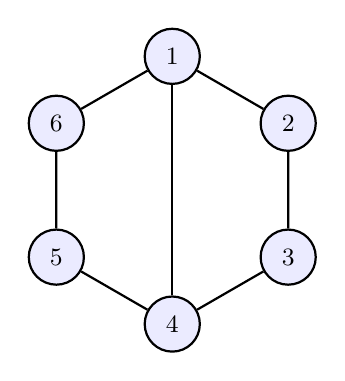
\begin{tikzpicture}[every node/.style={circle,draw,fill=blue!8,minimum size=7mm,font=\small},thick]
  \foreach \i/\ang in {1/90,2/30,3/-30,4/-90,5/-150,6/150}
    \node (v\i) at (\ang:1.7) {\i};
  \draw (v1)--(v2)--(v3)--(v4)--(v5)--(v6)--(v1);
  \draw (v1)--(v4);
\end{tikzpicture}
\end{center}

Process edges in order $12,23,34,45,56,61,14$.
\begin{itemize}
  \item $\{1,2\}$: both free $\Rightarrow$ match it, $S=\{1,2\}$.
  \item $\{2,3\}$: $2\in S$, skip.
  \item $\{3,4\}$: both free $\Rightarrow$ match, $S=\{1,2,3,4\}$.
  \item $\{4,5\}$: $4\in S$, skip. $\{5,6\}$: both free $\Rightarrow$ match, $S=\{1,2,3,4,5,6\}$.
  \item $\{6,1\}$: covered. $\{1,4\}$: covered.
\end{itemize}
Output $S=V$, size $6$, with $\abs M=3$. The optimum here is $\{1,3,5\}$? Check: edge $\{2,3\}$ has
$3$, $\{4,5\}$ has $5$, $\{6,1\}$ has $1$, $\{1,2\}$ has $1$, $\{3,4\}$ has $3$, $\{5,6\}$ has $5$,
chord $\{1,4\}$ has $1$ --- yes, size $3$ is optimal. So we returned $6 = 2\cdot 3$: the bound is
tight on this instance. The order of edges matters for the constant in practice, never for the
guarantee.
\end{labbox}

\begin{trapbox}
A tempting ``improvement'': repeatedly pick the \emph{highest-degree} vertex, add it to the cover,
delete it, repeat. This greedy-by-degree heuristic feels smarter --- and it is \emph{not} a constant
approximation. There are bipartite instances on which it returns a cover of size
$\Theta(\log n)\cdot\mathrm{OPT}$. The humble matching beats the clever greedy because the matching
hands us a matching lower bound; degree-greedy hands us nothing to compare against.
\end{trapbox}

\subsection{The LP relaxation and rounding}

The second route makes the lower bound explicit as a linear program, and it generalizes to weighted
vertex cover, where each vertex $v$ has cost $w_v\ge 0$ and we minimize total cost. Write a $0/1$
variable $x_v$ for ``$v$ is in the cover.''
\[
  \textbf{(IP)}\quad \min \sum_{v} w_v x_v
  \quad\text{s.t.}\quad x_u + x_v \ge 1\ \ \forall \{u,v\}\in E,\quad x_v\in\{0,1\}.
\]
Relax the integrality to $x_v\in[0,1]$ to get the LP. Its optimum $\mathrm{OPT}_{\mathrm{LP}}$ is a
lower bound on the integral optimum, since every integral solution is a feasible fractional one:
$\mathrm{OPT}_{\mathrm{LP}}\le\mathrm{OPT}$. Solve the LP (polynomial time), then \emph{round}: put
$v$ in the cover iff $x_v\ge \tfrac12$.

\begin{whybox}
\textbf{Feasibility.} For any edge, $x_u+x_v\ge 1$ forces $\max(x_u,x_v)\ge \tfrac12$, so at least
one endpoint is rounded up. Every edge is covered.

\textbf{Ratio.} Rounding up at $\tfrac12$ at most doubles each chosen coordinate:
$x_v\ge\tfrac12 \Rightarrow 1 \le 2x_v$. Therefore
\[
  \sum_{v\in S} w_v \;\le\; \sum_{v\in S} w_v\cdot 2x_v \;\le\; 2\sum_v w_v x_v
  \;=\; 2\,\mathrm{OPT}_{\mathrm{LP}} \;\le\; 2\,\mathrm{OPT}. \qquad\blacksquare
\]
\end{whybox}

This is the prototypical \emph{relax-and-round} argument: solve a tractable continuous relaxation,
then convert the fractional answer to an integral one while controlling the cost blow-up. The factor
$2$ here is exactly the ``threshold'' $1/\tfrac12$.

\begin{focusbox}
\textbf{Half-integrality (Nemhauser--Trotter).} For unweighted vertex cover the LP has a remarkable
property: there is always an optimal solution with every $x_v\in\{0,\tfrac12,1\}$. The variables at
$1$ are in \emph{every} optimal integral cover and the ones at $0$ are in none; only the $\tfrac12$
mass is genuinely undecided. This shrinks the problem to its ``hard core'' and is the seed of the
kernelization in the FPT chapter.
\end{focusbox}

\begin{connectionbox}
The LP dual of vertex cover is \emph{fractional matching}: $\max\sum_e y_e$ subject to
$\sum_{e\ni v} y_e\le 1$. LP duality says
$\mathrm{OPT}_{\mathrm{matching}}^{\mathrm{frac}}=\mathrm{OPT}_{\mathrm{VC}}^{\mathrm{frac}}$, and on
bipartite graphs both relaxations are integral (K\H{o}nig's theorem, Chapter on bipartite matching),
so vertex cover is \emph{exactly} solvable there. The factor-$2$ gap is a strictly non-bipartite
phenomenon --- the odd cycles are what cost us.
\end{connectionbox}

\begin{historybox}
Whether $2$ is the best constant possible is one of the famous open questions. Under the Unique Games
Conjecture, vertex cover is \textsf{NP}-hard to approximate within $2-\eps$ for every $\eps>0$
(Khot--Regev, 2003). Without UGC, the best hardness is $1.36$ (Dinur--Safra) improved toward
$\sqrt 2$. So the trivial matching algorithm may already be optimal --- we just cannot prove it.
\end{historybox}

\section{Set cover and the greedy $\ln n$ bound}

Vertex cover is a special case of \emph{set cover}, the canonical covering problem and the home of
the greedy method. Given a universe $U$ of $n$ elements and a family
$\mathcal{S}=\{S_1,\dots,S_m\}$ of subsets (with costs $c_i$, or unit cost in the simplest version)
whose union is $U$, find a minimum-cost subfamily covering $U$. On a graph, ``elements are edges,
sets are the edges incident to each vertex'' recovers vertex cover.

\begin{intuitionbox}
Greedy is the obvious idea: keep buying the set that covers the most still-uncovered elements per
dollar, until everything is covered. The surprise is the analysis. Greedy can be off by a factor of
$\ln n$ --- and that factor is essentially unavoidable for any polynomial algorithm. The proof is a
charging argument: spread each set's cost evenly over the new elements it covers, then sum the
harmonic series.
\end{intuitionbox}

\begin{algorithm}[H]
\caption{\textsc{GreedySetCover}$(U,\mathcal{S},c)$}\label{ch38:alg-setcover}
\DontPrintSemicolon
$C \gets \emptyset$;\quad $R \gets U$ \tcp*{$R$ = uncovered elements}
\While{$R \neq \emptyset$}{
  pick $S_i$ maximizing the coverage rate $\dfrac{\abs{S_i\cap R}}{c_i}$\;
  \ForEach{$e \in S_i\cap R$}{ price$(e) \gets \dfrac{c_i}{\abs{S_i\cap R}}$ }
  $C \gets C\cup\{i\}$;\quad $R \gets R\setminus S_i$\;
}
\Return $C$\;
\end{algorithm}

\begin{theorem}\label{ch38:thm-greedy-setcover}
\textsc{GreedySetCover} returns a cover of cost at most $H_n\cdot\mathrm{OPT}$, where
$H_n=\sum_{k=1}^n \tfrac1k \le \ln n + 1$.
\end{theorem}

\begin{whybox}
The total cost of greedy equals $\sum_{e\in U}\text{price}(e)$, because each set's cost is split
exactly among the new elements it pays for. So it suffices to bound the prices.

Fix an optimal cover $\mathcal{O}$ of cost $\mathrm{OPT}$. We claim
$\sum_{e\in S}\text{price}(e)\le H_{\abs S}\cdot c(S)$ for every set $S\in\mathcal{O}$. Order the
elements of $S$ by the time greedy covered them: $e_1,e_2,\dots,e_k$ ($k=\abs S$), most-recently
covered last. Consider the moment just before $e_j$ was covered. At that instant $e_j,\dots,e_k$ are
all still uncovered, so $S$ itself could cover at least $k-j+1$ of $R$ at rate
$c(S)/(k-j+1)$. Greedy chose a set at least this cost-effective, so the price charged to $e_j$
satisfies
\[
  \text{price}(e_j) \;\le\; \frac{c(S)}{k-j+1}.
\]
Summing over $j=1,\dots,k$ gives $\sum_{e\in S}\text{price}(e)\le c(S)\,H_k$. Now sum over the optimal
sets, and note each element is in at least one optimal set:
\[
  \text{greedy cost} = \sum_{e}\text{price}(e) \le \sum_{S\in\mathcal{O}}\sum_{e\in S}\text{price}(e)
  \le H_n \sum_{S\in\mathcal{O}} c(S) = H_n\cdot\mathrm{OPT}. \qquad\blacksquare
\]
\end{whybox}

\begin{labbox}
Tiny unit-cost instance. Universe $U=\{1,2,3,4,5,6\}$, sets
\[
  A=\{1,2,3,4\},\quad B=\{1,2,5\},\quad C=\{3,4,6\},\quad D=\{5,6\}.
\]

\begin{center}
\begin{tikzpicture}[thick,
  elt/.style={circle,draw,fill=blue!8,minimum size=5mm,inner sep=0pt,font=\footnotesize},
  setn/.style={font=\small\bfseries}]
  \foreach \e/\x in {1/0,2/1,3/2,4/3,5/4,6/5} \node[elt] (e\e) at (\x,0) {\e};
  \node[setn] (A) at (1.5,1.5) {$A$};
  \node[setn] (B) at (0.5,-1.5) {$B$};
  \node[setn] (C) at (2.5,-1.5) {$C$};
  \node[setn] (D) at (4.5,-1.5) {$D$};
  \foreach \e in {1,2,3,4} \draw[sourceblue] (A)--(e\e);
  \foreach \e in {1,2,5} \draw[targetgreen] (B)--(e\e);
  \foreach \e in {3,4,6} \draw[quotientorange] (C)--(e\e);
  \foreach \e in {5,6} \draw[structurepurple] (D)--(e\e);
\end{tikzpicture}
\end{center}

Greedy first compares coverage: $\abs A=4$ wins. Pick $A$; remaining $R=\{5,6\}$. Now
$\abs{B\cap R}=1$, $\abs{C\cap R}=1$, $\abs{D\cap R}=2$. Pick $D$; done. Greedy returns $\{A,D\}$,
cost $2$ --- which is optimal here, so greedy was lucky. The classic bad instance stacks two big
sets each covering ``half plus one'' against the cheap optimal pair, forcing the harmonic loss; build
it in Exercise~\ref{ch38:ex-setcover-tight}.
\end{labbox}

\begin{complexitybox}
With a priority queue keyed by current coverage, greedy runs in $\Oh\!\left(\sum_i \abs{S_i}\log m\right)$.
The $\ln n$ ratio is tight: Feige (1998) proved set cover is \textsf{NP}-hard to approximate within
$(1-o(1))\ln n$, so greedy is essentially optimal among all polynomial algorithms. Few problems pin
down their approximability so precisely.
\end{complexitybox}

\section{Metric TSP, the double-tree bound, and Christofides}

The traveling salesman problem: given a complete graph on $V$ with edge weights $w$, find a minimum
weight Hamiltonian cycle (a tour visiting every vertex once and returning). General TSP cannot be
approximated within any constant unless $\textsf{P}=\textsf{NP}$ (a tour-or-no-tour gadget makes even
a ratio-$2^{\poly}$ approximation \textsf{NP}-hard). The fix is the \emph{metric} assumption: weights
satisfy the triangle inequality $w(u,w)\le w(u,v)+w(v,w)$. This is exactly the regime of real
distances, and it is approximable.

\subsection{The MST lower bound and double-tree}

\begin{intuitionbox}
Delete one edge from a tour and you have a Hamiltonian \emph{path} --- a spanning tree (a very thin
one). So every tour contains a spanning tree, giving
\[
  \mathrm{MST} \;\le\; \mathrm{OPT}.
\]
That is the lower bound. To turn a tree into a tour, walk around it (an Euler-tour traversal visiting
each edge twice) and then ``shortcut'' past already-visited vertices. The walk costs $2\,\mathrm{MST}$;
shortcutting only helps because of the triangle inequality. Result: a $2$-approximation.
\end{intuitionbox}

\begin{algorithm}[H]
\caption{\textsc{DoubleTreeTSP}$(\Gph,w)$ -- metric}\label{ch38:alg-doubletree}
\DontPrintSemicolon
$T \gets$ minimum spanning tree of $\Gph$\;
$T' \gets$ multigraph doubling every edge of $T$ \tcp*{all degrees even}
$W \gets$ Eulerian circuit of $T'$ \tcp*{exists: connected, even degrees}
walk $W$, output vertices in first-visit order, close the cycle\;
\Return the resulting Hamiltonian tour\;
\end{algorithm}

\begin{whybox}
$T'$ is connected and every vertex has even degree (each tree edge contributes $2$), so an Eulerian
circuit exists and has weight $2\,\mathrm{MST}$. Reading off first visits and shortcutting replaces a
detour $u\to\cdots\to v$ by the direct edge $u\to v$; the triangle inequality (applied repeatedly)
guarantees the direct edge is no longer than the path it replaces. So the tour weighs at most
$2\,\mathrm{MST}\le 2\,\mathrm{OPT}$.
\end{whybox}

\begin{figure}[H]
\centering
\begin{tikzpicture}[every node/.style={circle,draw,fill=green!8,minimum size=6mm,inner sep=1pt,font=\small},thick]
  \node (r) at (0,1.4) {$r$};
  \node (a) at (-1.6,0) {$a$};
  \node (b) at (1.6,0) {$b$};
  \node (c) at (-1.6,-1.4) {$c$};
  \node (d) at (1.6,-1.4) {$d$};
  \draw[sourceblue,very thick] (r)--(a); \draw[sourceblue,very thick] (r)--(b);
  \draw[sourceblue,very thick] (a)--(c); \draw[sourceblue,very thick] (b)--(d);
  \draw[quotientorange,dashed,bend left=55] (c) to node[draw=none,fill=none,below left,font=\footnotesize]{shortcut} (d);
\end{tikzpicture}
\caption{Double-tree on a small MST (solid). The Euler walk
$r\,a\,c\,a\,r\,b\,d\,b\,r$ traverses each tree edge twice; reading off first
visits $r,a,c,b,d$ and closing the cycle replaces the back-tracking
$c\to a\to r\to b\to d$ by the direct shortcut $c\to d$ (dashed), which the
triangle inequality keeps no longer.}
\label{ch38:fig-doubletree}
\end{figure}

\subsection{Christofides: fixing the parity instead of doubling}

Doubling every edge is wasteful: we double the \emph{whole} tree just to make degrees even, but only
the odd-degree vertices were a problem. Christofides' insight is to repair parity with a minimum
\emph{matching} on exactly those vertices.

\begin{focusbox}
A graph has an Eulerian circuit iff it is connected and \emph{every vertex has even degree}. In the
MST $T$, let $O$ be the set of odd-degree vertices. A classical fact (handshake lemma) says $\abs O$
is even. Add a minimum-weight perfect matching $M$ on $O$ (using the metric distances): each vertex
of $O$ gains exactly one edge, flipping its parity to even, while even-degree vertices are untouched.
Now $T\cup M$ is Eulerian.
\end{focusbox}

\begin{algorithm}[H]
\caption{\textsc{Christofides}$(\Gph,w)$ -- metric}\label{ch38:alg-christofides}
\DontPrintSemicolon
$T \gets$ minimum spanning tree\;
$O \gets$ vertices of odd degree in $T$ \tcp*{$\abs O$ even}
$M \gets$ minimum-weight perfect matching on $O$ (metric weights)\;
$H \gets T \cup M$ \tcp*{multigraph; all degrees even, connected}
$W \gets$ Eulerian circuit of $H$\;
shortcut $W$ to a Hamiltonian tour and return it\;
\end{algorithm}

\begin{theorem}\label{ch38:thm-christofides}
\textsc{Christofides} is a $\tfrac32$-approximation for metric TSP.
\end{theorem}

\begin{whybox}
The Eulerian circuit weighs $w(T)+w(M)$, and shortcutting only decreases weight, so the tour costs at
most $w(T)+w(M)$. We bound each piece against $\mathrm{OPT}$.

\emph{Tree:} $w(T)=\mathrm{MST}\le\mathrm{OPT}$, as before.

\emph{Matching:} This is the clever part. Take an optimal tour and restrict attention to the vertices
$O$, visited by the tour in some cyclic order $o_1,o_2,\dots,o_{2t},o_1$. Shortcutting the tour onto
just these vertices gives a cycle $\mathcal{C}$ on $O$ of weight at most $\mathrm{OPT}$ (triangle
inequality). An even cycle splits into two perfect matchings --- the odd-indexed edges and the
even-indexed edges --- whose weights sum to $w(\mathcal{C})\le\mathrm{OPT}$. The cheaper of the two
weighs at most $\tfrac12\mathrm{OPT}$, and the minimum perfect matching $M$ is no heavier:
\[
  w(M) \;\le\; \tfrac12\,\mathrm{OPT}.
\]
Adding up: tour weight $\le w(T)+w(M)\le \mathrm{OPT}+\tfrac12\mathrm{OPT}=\tfrac32\mathrm{OPT}$.
$\blacksquare$
\end{whybox}

\begin{labbox}
Four points on a line (a metric): $a=0, b=1, c=2, d=4$, distances $=$ absolute differences. The MST is
the path $a\!-\!b\!-\!c\!-\!d$, weight $1+1+2=4$. Odd-degree vertices: the two endpoints $a$ and $d$
(degree $1$); $b,c$ have degree $2$.

\begin{center}
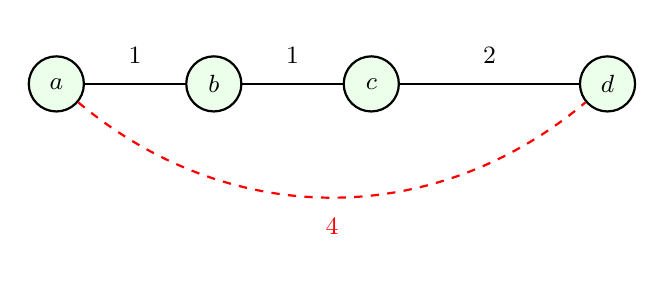
\begin{tikzpicture}[every node/.style={circle,draw,fill=green!8,minimum size=7mm,font=\small},thick]
  \node (a) at (0,0) {$a$};
  \node (b) at (2,0) {$b$};
  \node (c) at (4,0) {$c$};
  \node (d) at (7,0) {$d$};
  \draw (a)--node[above,draw=none,fill=none]{$1$}(b);
  \draw (b)--node[above,draw=none,fill=none]{$1$}(c);
  \draw (c)--node[above,draw=none,fill=none]{$2$}(d);
  \draw[red,dashed,bend right=40] (a) to node[below,draw=none,fill=none]{\color{red}$4$} (d);
\end{tikzpicture}
\end{center}

The minimum matching on $O=\{a,d\}$ is just the single edge $\{a,d\}$ of weight $4$ (red, dashed).
Then $H = T\cup\{ad\}$ is a cycle $a\!-\!b\!-\!c\!-\!d\!-\!a$, already Hamiltonian, weight
$4+4=8$. The optimal tour visits $a,b,c,d$ in order and returns: $1+1+2+4=8$ too. So on this instance
Christofides is exact. (Double-tree would have produced the Eulerian walk of weight $2\cdot4=8$ and
shortcut to the same $8$ --- the gap between the methods shows only when the odd set is small relative
to the tree.)
\end{labbox}

\begin{historybox}
Christofides published the $3/2$ bound in 1976; it stood untouched as the best known ratio for metric
TSP for \emph{forty-four years}. In 2020, Karlin, Klein, and Oveis Gharan broke it by
$10^{-36}$ using a randomized maximum-entropy distribution over spanning trees --- a result whose
importance is entirely conceptual, proving the $3/2$ barrier was not fundamental. For the special
case of graph metrics the bound is now $1.4$ (Seb\H{o}--Vygen). The bottleneck is the matching step:
making it interact with the tree, rather than be chosen afterward, is the modern frontier.
\end{historybox}

\begin{complexitybox}
MST is $\Oh(n^2)$ on a dense metric (Prim with arrays). The matching dominates: a minimum-weight
perfect matching on $\abs O\le n$ vertices via blossom-based methods costs $\Oh(n^3)$. So
Christofides is $\Oh(n^3)$. Double-tree is only $\Oh(n^2\log n)$ but gives the weaker factor $2$.
\end{complexitybox}

\section{Steiner tree: the metric closure and double-spanning-tree}

\emph{Steiner tree} generalizes MST. We are given a graph (or metric) and a subset $R\subseteq V$ of
\emph{terminals}; we must connect all terminals as cheaply as possible, but we are \emph{allowed} to
route through non-terminal \emph{Steiner} vertices. Minimizing over which Steiner vertices to use is
what makes it \textsf{NP}-hard. The natural $2$-approximation reuses the doubling idea on the
\emph{metric closure}.

\begin{intuitionbox}
Pretend the Steiner vertices do not exist: build the complete graph on the terminals $R$, where the
weight of $\{s,t\}$ is the shortest-path distance $\dist(s,t)$ in the original graph. Compute an MST
of \emph{that}. Expand each chosen ``metric edge'' back into its underlying shortest path. The result
connects all terminals, possibly using Steiner vertices for free as waypoints, and the doubling
argument bounds it by twice the optimum.
\end{intuitionbox}

\begin{algorithm}[H]
\caption{\textsc{SteinerMST}$(\Gph,w,R)$}\label{ch38:alg-steiner}
\DontPrintSemicolon
compute the metric closure $\bar\Gph$ on $R$: $\bar w(s,t)=\dist_\Gph(s,t)$\;
$\bar T \gets$ minimum spanning tree of $\bar\Gph$\;
replace each edge $\{s,t\}\in\bar T$ by a shortest $s$--$t$ path in $\Gph$\;
remove cycles/redundant edges to get a tree; \Return it\;
\end{algorithm}

\begin{theorem}\label{ch38:thm-steiner2}
\textsc{SteinerMST} returns a Steiner tree of weight at most $2(1-\tfrac1{\abs R})\,\mathrm{OPT}<2\,\mathrm{OPT}$.
\end{theorem}

\begin{whybox}
Let $T^\ast$ be an optimal Steiner tree, weight $\mathrm{OPT}$. Double its edges and take an Eulerian
circuit $W$ of weight $2\,\mathrm{OPT}$. Walk $W$ and shortcut to the terminals in order of first
visit: this yields a Hamiltonian cycle $\mathcal{H}$ \emph{on the terminals only}, where consecutive
terminals are joined by direct metric edges. Each such metric edge is at most the length of the path
it shortcut (paths in $W$ are at least metric distances), so $\bar w(\mathcal{H})\le 2\,\mathrm{OPT}$.
Deleting the heaviest edge of $\mathcal{H}$ leaves a spanning \emph{path} of the terminals in
$\bar\Gph$, hence a spanning tree, of weight $\le 2\,\mathrm{OPT}$. The MST $\bar T$ is no heavier, so
$\bar w(\bar T)\le 2\,\mathrm{OPT}$, and expanding edges to paths does not increase weight. The
$(1-1/\abs R)$ refinement comes from deleting the heaviest of $\abs R$ cycle edges, which is at least
the average. $\blacksquare$
\end{whybox}

\begin{labbox}
A ``plus sign'': central Steiner vertex $c$ joined to four terminals $N,S,E,W$ each at distance $1$;
the terminals are pairwise at distance $2$ through $c$ (or directly, say, also $2$). Metric closure on
$\{N,S,E,W\}$ has all weights $2$; its MST is any spanning tree, weight $3\cdot 2 = 6$. Expanding,
e.g., the path $N\!-\!E\!-\!S\!-\!W$ routes through $c$ and reuses the spoke to $c$. But the true
optimum is the star: four spokes of weight $1$, total $4$. So this algorithm returns $6 \le 2\cdot 4$,
illustrating both the looseness and the role of the unused Steiner vertex. The famous worst case is
the star, where ignoring Steiner points costs the full factor $2(1-1/\abs R)$.
\end{labbox}

\begin{connectionbox}
The integrality gap of this MST relaxation is exactly $2$, but better relaxations exist. The
bidirected-cut and hypergraph LPs, rounded by the iterative ``loss-contracting'' algorithm of
Byrka--Grandoni--Rothvo\ss--Sanit\`a (2010), achieve $\ln 4 + \eps \approx 1.39$, the current best.
The jump from combinatorial $2$ to LP-based $1.39$ mirrors the vertex-cover and TSP stories: a sharper
lower bound buys a sharper ratio.
\end{connectionbox}

\section{Max-cut: greedy, local search, and the SDP leap}

Now a maximization problem. Given $\Gph=(V,E)$ (unit weights for simplicity), partition $V$ into
$(A,B)$ to maximize the number of \emph{cut} edges --- edges with one endpoint on each side. Max-cut
is \textsf{NP}-hard, in sharp contrast to min-cut, which is polynomial.

\subsection{Greedy and local search: factor one half}

\begin{intuitionbox}
A coin flip already does well. Put each vertex on side $A$ or $B$ independently with probability
$\tfrac12$. An edge is cut with probability $\tfrac12$, so the expected cut size is $\tfrac12\abs E$.
Since $\mathrm{OPT}\le\abs E$, this is a $\tfrac12$-approximation \emph{in expectation}. Local search
derandomizes it: while some vertex has more edges to its own side than across, flip it. Each flip
strictly increases the cut, so it terminates, and at the end every vertex has at least half its edges
cut --- summing gives a cut of $\ge\tfrac12\abs E$.
\end{intuitionbox}

\begin{algorithm}[H]
\caption{\textsc{LocalMaxCut}$(\Gph)$}\label{ch38:alg-localcut}
\DontPrintSemicolon
$(A,B)\gets$ arbitrary partition\;
\While{some $v$ has more neighbors on its own side than the other}{
  move $v$ to the other side\;
}
\Return $(A,B)$\;
\end{algorithm}

\begin{whybox}
Let $d(v)$ be $v$'s degree and $c(v)$ the number of its edges currently cut. At a local optimum
$c(v)\ge d(v)/2$ for all $v$ (else flipping $v$ improves). Summing, $\sum_v c(v)\ge\tfrac12\sum_v
d(v)$. Each cut edge is counted twice on the left and each edge twice on the right, so
$2\,\abs{\text{cut}}\ge \abs E$, i.e.\ the cut has $\ge\abs E/2\ge\mathrm{OPT}/2$ edges. Each flip
raises the integer cut value by at least $1$, and the cut is bounded by $\abs E$, so at most $\abs E$
flips occur: $\Oh(\abs V\abs E)$ time. $\blacksquare$
\end{whybox}

\subsection{Goemans--Williamson: the $0.878$ SDP rounding}

The factor $\tfrac12$ feels weak --- and it is. The breakthrough is to relax to a
\emph{semidefinite} program. Encode each vertex as a unit vector $x_v\in\R^n$ and replace the discrete
$\pm 1$ assignment by geometry on the unit sphere.

\begin{intuitionbox}
For a $\pm1$ labeling $y_v$, the indicator ``$\{u,v\}$ is cut'' equals $\tfrac{1-y_uy_v}{2}$. Lift
$y_v\in\{\pm1\}$ to a unit \emph{vector} $x_v$ and replace the product $y_uy_v$ by the inner product
$\langle x_u,x_v\rangle$. Maximizing $\sum_{\{u,v\}\in E}\tfrac{1-\langle x_u,x_v\rangle}{2}$ over unit
vectors is a relaxation (the $1$-dimensional $\pm1$ case is a feasible point), and crucially it is
\emph{solvable} --- it is a semidefinite program in the Gram matrix $X_{uv}=\langle x_u,x_v\rangle$,
which must be positive semidefinite. Then we round by a random hyperplane: pick a uniformly random
direction $r$ and split vertices by the sign of $\langle x_v, r\rangle$.
\end{intuitionbox}

\begin{center}
\begin{tikzpicture}[scale=1.6,thick]
  \draw[gray!50] (0,0) circle (1);
  \coordinate (O) at (0,0);
  \coordinate (xu) at (40:1);
  \coordinate (xv) at (135:1);
  \draw[->,sourceblue,very thick] (O)--(xu) node[above right]{$x_u$};
  \draw[->,targetgreen,very thick] (O)--(xv) node[above left]{$x_v$};
  \draw[red,dashed] (-1.2,0.5) -- (1.2,-0.5) node[right,draw=none]{\color{red} hyperplane $r^\perp$};
  \draw pic[draw,angle radius=0.5cm,"$\theta$",angle eccentricity=1.4] {angle=xu--O--xv};
\end{tikzpicture}
\end{center}

A random hyperplane separates $x_u$ and $x_v$ exactly when it falls in the angle $\theta$ between
them, which happens with probability $\theta/\pi$.

\begin{algorithm}[H]
\caption{\textsc{GW-MaxCut}$(\Gph)$}\label{ch38:alg-gw}
\DontPrintSemicolon
solve the SDP: $\max \sum_{\{u,v\}\in E}\dfrac{1-\langle x_u,x_v\rangle}{2}$ over unit vectors $x_v\in\R^n$\;
draw a random Gaussian vector $r\in\R^n$\;
$A \gets \{v: \langle x_v, r\rangle \ge 0\}$,\quad $B \gets V\setminus A$\;
\Return $(A,B)$\;
\end{algorithm}

\begin{theorem}[Goemans--Williamson, 1995]\label{ch38:thm-gw}
\textsc{GW-MaxCut} returns a cut of expected value at least $\alpha_{\mathrm{GW}}\cdot\mathrm{OPT}$,
where
\[
  \alpha_{\mathrm{GW}} = \min_{0\le\theta\le\pi}\frac{\theta/\pi}{(1-\cos\theta)/2}
  \;\approx\; 0.87856.
\]
\end{theorem}

\begin{whybox}
For an edge with vectors at angle $\theta_{uv}=\arccos\langle x_u,x_v\rangle$, the probability the
random hyperplane cuts it is exactly $\theta_{uv}/\pi$ (the fraction of directions whose hyperplane
falls between the two vectors). The edge's contribution to the SDP objective is
$(1-\cos\theta_{uv})/2$. The pointwise ratio is bounded below by the constant
$\alpha_{\mathrm{GW}}=\min_\theta \frac{\theta/\pi}{(1-\cos\theta)/2}$, so by linearity of
expectation,
\[
  \mathbb{E}[\text{cut}] = \sum_{\{u,v\}\in E}\frac{\theta_{uv}}{\pi}
  \;\ge\; \alpha_{\mathrm{GW}}\sum_{\{u,v\}\in E}\frac{1-\cos\theta_{uv}}{2}
  = \alpha_{\mathrm{GW}}\cdot\mathrm{SDP}
  \;\ge\; \alpha_{\mathrm{GW}}\cdot\mathrm{OPT}.
\]
The minimizing angle is near $\theta^\ast\approx 2.331$ rad ($134^\circ$), where the ratio bottoms out
at $\approx 0.87856$. $\blacksquare$
\end{whybox}

\begin{trapbox}
The ratio is \emph{not} achieved at the endpoints. At $\theta=\pi$ (antipodal vectors) it equals $1$;
as $\theta\to 0$ the ratio $\frac{2\theta}{\pi(1-\cos\theta)}$ actually \emph{diverges} to $+\infty$,
since the denominator $1-\cos\theta\sim\theta^2/2$ shrinks faster than the numerator. The worst case
is the interior angle $\approx 134^\circ$. A common error is to ``bound'' the ratio by checking
endpoints; you must minimize over the whole interval. Plot $f(\theta)=\frac{2\theta}{\pi(1-\cos\theta)}$
to see the single interior minimum.
\end{trapbox}

\begin{historybox}
Before 1995 the best max-cut ratio was the trivial $1/2$ (with lower-order additive improvements). GW
shattered it and, with it, launched SDP as a core tool of approximation. The number $0.87856$ turned
out to be \emph{exactly} optimal: under the Unique Games Conjecture, beating
$\alpha_{\mathrm{GW}}$ is \textsf{NP}-hard (Khot--Kindler--Mossel--O'Donnell, 2007). The hardness
constant is the \emph{same} transcendental number that falls out of the rounding analysis --- a
striking coincidence of upper and lower bounds.
\end{historybox}

\begin{complexitybox}
The SDP solves to additive error $\delta$ in time $\poly(n,\log\tfrac1\delta)$ via interior-point or
the matrix-multiplicative-weights method; the rounding is $\Oh(n^2)$ for the dot products. Expected
ratio $0.878$; it can be made high-probability by repeating the hyperplane draw $\Oh(\log n)$ times
and keeping the best cut.
\end{complexitybox}

\begin{connectionbox}
The SDP relaxation is an \emph{eigenvalue}-flavored object: writing it in the Laplacian $\Lap$, the
spectral relaxation $\frac14\lambda_{\max}(\Lap)\cdot$(a balance term) is a looser cousin, and the
SDP is the tightest convex relaxation invariant under rotations. This is the same Laplacian whose
\emph{small} eigenvalues govern sparsest cut below and whose spectrum threads the spectral-graph and
expander chapters. Max-cut wants the top of the spectrum; conductance wants the bottom.
\end{connectionbox}

\section{Sparsest cut, conductance, and the Leighton--Rao / ARV story}

We end with the deepest problem in the chapter, the one that connects approximation to spectra, metric
embeddings, and electrical flows. The \emph{sparsest cut} asks for the partition that is cheap in
edges \emph{and} balanced in vertices.

\begin{definition}[Sparsest cut / conductance]\label{ch38:def-sparsest}
For $S\subseteq V$ with $0<\abs S\le \abs V/2$, the (uniform, or edge-) \emph{sparsity} is
\[
  \Phi(S) = \frac{\abs{E(S,\bar S)}}{\abs S\,\abs{\bar S}},
  \qquad\text{and the related \emph{conductance}}\quad
  \phi(S) = \frac{\abs{E(S,\bar S)}}{\min(\mathrm{vol}(S),\mathrm{vol}(\bar S))},
\]
where $\mathrm{vol}(S)=\sum_{v\in S}\deg(v)$. The sparsest cut is $\min_S\Phi(S)$; the
\emph{Cheeger constant} (edge expansion) is $\min_S \phi(S)$.
\end{definition}

\begin{intuitionbox}
Min-cut alone is fooled by a single pendant vertex: cutting it off costs one edge and is ``sparse''
but useless for clustering --- it isolates almost nothing. Dividing by $\abs S\abs{\bar S}$ (or by the
volume) \emph{rewards balance}, so the sparsest cut finds the genuine bottleneck of the graph: the
dumbbell's thin neck, the two communities' weak interface. This is exactly the cut you want for
divide-and-conquer, image segmentation, and clustering --- and it is \textsf{NP}-hard to compute
exactly.
\end{intuitionbox}

\begin{center}
\begin{tikzpicture}[every node/.style={circle,draw,fill=blue!8,minimum size=5mm,inner sep=1pt,font=\footnotesize},thick]
  \foreach \i in {1,2,3} \node (l\i) at (0,{-\i*0.8}) {};
  \node (l4) at (-0.8,-1.6) {};
  \foreach \i in {1,2,3} \node (r\i) at (4,{-\i*0.8}) {};
  \node (r4) at (4.8,-1.6) {};
  \foreach \i in {1,2,3,4}\foreach \j in {1,2,3,4}{\ifnum\i<\j \draw[edgegray] (l\i)--(l\j);\fi}
  \foreach \i in {1,2,3,4}\foreach \j in {1,2,3,4}{\ifnum\i<\j \draw[edgegray] (r\i)--(r\j);\fi}
  \draw[red,very thick] (l2)--(r2);
  \node[draw=none,fill=none,red] at (2,-0.5) {thin neck};
\end{tikzpicture}
\end{center}

\subsection{The spectral bound (Cheeger) and where it fails}

The bottom of the Laplacian spectrum gives a fast two-sided estimate. With $\lambda_2$ the second
smallest eigenvalue of the normalized Laplacian, \emph{Cheeger's inequality} reads
\[
  \frac{\lambda_2}{2} \;\le\; \phi_G \;\le\; \sqrt{2\lambda_2}.
\]
Computing $\lambda_2$ and rounding its eigenvector (the ``sweep cut'') gives a cut within a
\emph{quadratic} factor of optimal --- excellent when $\phi$ is constant, but as bad as $\Oh(1/\phi)$
when the graph is a near-expander. The full development lives in the spectral and expander chapters;
here we only note its place as the cheapest sparsest-cut approximation.

\subsection{Leighton--Rao: LP, multicommodity flow, and $\Oh(\log n)$}

\begin{intuitionbox}
The LP relaxation of sparsest cut assigns a \emph{distance} $d_{uv}\ge 0$ to each pair, forming a
metric ($d$ obeys the triangle inequality), minimizing $\sum_{\{u,v\}\in E} d_{uv}$ subject to total
spread $\sum_{u,v} d_{uv}=1$. By LP duality this equals the maximum \emph{concurrent multicommodity
flow} --- route a unit of flow between every pair without exceeding edge capacities. The flow/cut gap
is what we must round.

The rounding theorem (Linial--London--Rabinovich; Bourgain): \emph{every $n$-point metric embeds into
$\ell_1$ with distortion $\Oh(\log n)$}. An $\ell_1$ metric is a nonnegative combination of cut
metrics, and a cut metric is an actual cut. So we solve the LP, embed the optimal metric into
$\ell_1$ losing a factor $\Oh(\log n)$, and read off a cut.
\end{intuitionbox}

\begin{theorem}[Leighton--Rao, 1988]\label{ch38:thm-lr}
There is a polynomial-time $\Oh(\log n)$-approximation for sparsest cut, via the LP relaxation and
Bourgain's $\ell_1$ embedding. Equivalently, the max-concurrent-flow / min-sparsest-cut gap is
$\Theta(\log n)$ for general demands.
\end{theorem}

\begin{whybox}
\emph{Why $\ell_1$ is the right target.} A cut $(S,\bar S)$ induces the \emph{cut metric}
$\delta_S(u,v)=\mathbf{1}[\,\text{$u,v$ on opposite sides}\,]$. Sparsity evaluated on a cut metric is
literally $\Phi(S)$. The set of $\ell_1$-embeddable metrics is exactly the cone spanned by cut
metrics, so optimizing sparsity over $\ell_1$ metrics \emph{is} optimizing over (distributions of)
cuts --- no gap. The only loss is squeezing the LP's arbitrary metric into $\ell_1$, and Bourgain's
theorem caps that loss at $\Oh(\log n)$. The matching lower bound (expanders give an
$\Omega(\log n)$ flow/cut gap) shows $\Oh(\log n)$ is best possible \emph{for this LP}. $\blacksquare$
\end{whybox}

\begin{focusbox}
\textbf{Bourgain's embedding, in one breath.} To embed a metric $(V,d)$ into $\ell_1$, pick
$\Oh(\log^2 n)$ random subsets $A$ of $V$ (at geometric scales of size) and map each vertex $v$ to the
vector of its distances $d(v,A)=\min_{a\in A}d(v,a)$, scaled. Distances contract by at most $1$ and,
in expectation across scales, expand by at least $\Omega(1/\log n)$ --- giving distortion
$\Oh(\log n)$. The random subsets are doing exactly what random hyperplanes did for GW: turning a
geometric object into combinatorial cuts.
\end{focusbox}

\subsection{ARV: the SDP and $\Oh(\sqrt{\log n})$}

\begin{intuitionbox}
Leighton--Rao uses an LP (a metric). Arora--Rao--Vazirani (2004) tighten it to an \emph{SDP}: embed
vertices as vectors $x_v$ with the extra constraint that squared distances $\norm{x_u-x_v}^2$
themselves form a metric (the metric is ``of negative type,'' i.e.\ $\ell_2^2$). This rules out the
degenerate configurations that cost Leighton--Rao a full $\log n$.

The heart is a geometric \emph{structure theorem}: in any such SDP solution, either there is an
obvious sparse cut, or one can find two large, $\Omega(1/\sqrt{\log n})$-separated sets of vertices
--- $\Delta$-separated ``well-spread'' sets --- whose existence forces a good cut. Chaining these
yields the bound.
\end{intuitionbox}

\begin{theorem}[Arora--Rao--Vazirani, 2004]\label{ch38:thm-arv}
The $\ell_2^2$ (negative-type) SDP gives an $\Oh(\sqrt{\log n})$-approximation for (uniform) sparsest
cut, and the integrality gap of that SDP is $\Omega(\log\log n)$ but $o(\log n)$.
\end{theorem}

We will not prove ARV --- its structure theorem and the
$\ell_2^2\!\hookrightarrow\!\ell_1$ embedding with distortion $\Oh(\sqrt{\log n})$ (Arora--Lee--Naor)
are a chapter unto themselves. The takeaway is the ladder of relaxations and ratios.

\begin{center}
\begin{tabular}{lll}
\toprule
Relaxation & Object & Sparsest-cut ratio \\
\midrule
Spectral (Cheeger) & eigenvector of $\Lap$ & quadratic ($\sqrt{\,\cdot\,}$ in $\phi$) \\
Leighton--Rao (LP) & arbitrary metric $\to\ell_1$ & $\Oh(\log n)$ \\
Arora--Rao--Vazirani (SDP) & $\ell_2^2$ metric $\to\ell_1$ & $\Oh(\sqrt{\log n})$ \\
\bottomrule
\end{tabular}
\end{center}

\begin{connectionbox}
This ladder is the spine of the rest of the book. The spectral row is the Laplacian and
expander-graph chapters; the eigenvector sweep is literally spectral clustering. The flow side of
Leighton--Rao duality is multicommodity flow, and the fast solvers that make ARV-style SDPs practical
run on \emph{electrical flows} and near-linear-time Laplacian system solvers --- the Spielman--Teng
machinery of the final chapter. Sparsest cut is where combinatorial optimization, convex geometry, and
spectral graph theory meet.
\end{connectionbox}

\begin{historybox}
Leighton and Rao's 1988 $\Oh(\log n)$ result was the first to break the spectral barrier with a
\emph{provable} guarantee for general graphs and seeded the whole metric-embedding program in
theoretical CS. ARV in 2004 was a landmark not just for the $\sqrt{\log n}$ ratio but for the
\emph{techniques}: measure concentration on the sphere and chaining arguments imported wholesale into
algorithm design. Whether sparsest cut admits a constant-factor approximation remains open and is tied
to the Unique Games Conjecture.
\end{historybox}

\section{A unifying picture}

Step back and the methods line up by the kind of lower bound they invent.

\begin{center}
\begin{tabular}{llll}
\toprule
Problem & Ratio & Lower bound used & Method \\
\midrule
Vertex cover & $2$ & maximal matching / LP & combinatorial / round \\
Set cover & $\ln n$ & fractional / charging & greedy \\
Metric TSP & $3/2$ & MST $+$ matching & Christofides \\
Steiner tree & $2$ ($1.39$) & metric-closure MST & double tree / LP \\
Max-cut & $0.878$ & SDP (Gram matrix) & hyperplane round \\
Sparsest cut & $\Oh(\sqrt{\log n})$ & LP / SDP metric & embed to $\ell_1$ \\
\bottomrule
\end{tabular}
\end{center}

\begin{aestheticbox}
Notice the trajectory. Combinatorial lower bounds (matchings, trees) give clean small constants but
plateau. LP relaxations match or beat them and expose duality. SDP relaxations --- the geometric leap
--- crack the problems where LPs have an inherent $\log n$ gap. And every single ratio has a matching
hardness result, often the \emph{same constant}, telling us the relaxation was not merely convenient
but \emph{exactly as powerful as polynomial computation allows}. That correspondence, relaxation
strength $=$ approximability, is the deepest lesson of the area.
\end{aestheticbox}

\section{Exercises}

\begin{exercise}\label{ch38:ex-vc-tight}
Show that Algorithm~\ref{ch38:alg-vc-match} can return exactly $2\,\mathrm{OPT}$ by exhibiting an
infinite family of graphs (hint: disjoint single edges, or a perfect matching) where it does. Then
argue no analysis of this algorithm can beat the constant $2$.
\end{exercise}

\begin{exercise}\label{ch38:ex-vc-weighted}
Implement the LP-rounding weighted vertex cover and verify the $2$-approximation on the weighted
$5$-cycle with vertex weights $1,2,1,2,1$. What does the LP optimum equal, and which vertices get
fractional value $\tfrac12$?
\end{exercise}

\begin{exercise}\label{ch38:ex-setcover-tight}
Construct, for each $k$, a unit-cost set-cover instance on $n=2^{k+1}-2$ elements where greedy returns
$k$ sets but the optimum is $2$. Conclude the analysis of
Theorem~\ref{ch38:thm-greedy-setcover} is tight up to a constant. (Hint: two ``optimal'' sets each of
size $n/2$, plus a chain of greedily-tempting sets of sizes $n/2, n/4, n/8,\dots$.)
\end{exercise}

\begin{exercise}\label{ch38:ex-christofides-tight}
Build a metric instance where Christofides returns a tour of weight approaching
$\tfrac32\mathrm{OPT}$. (Hint: a long path with a carefully placed extra vertex so the odd set is
$\{$two endpoints$\}$ and the matching edge is expensive.) Then trace both
Algorithm~\ref{ch38:alg-doubletree} and Algorithm~\ref{ch38:alg-christofides} on it.
\end{exercise}

\begin{exercise}\label{ch38:ex-tsp-nonmetric}
Prove that for \emph{general} (non-metric) TSP, the existence of a polynomial $\alpha$-approximation
for any constant $\alpha$ would imply $\textsf{P}=\textsf{NP}$. (Reduce from Hamiltonian cycle: weight
$1$ on graph edges, weight $\alpha n + 1$ on non-edges.)
\end{exercise}

\begin{exercise}\label{ch38:ex-steiner-gap}
Show the metric-closure MST relaxation for Steiner tree has integrality gap exactly
$2-\tfrac2{\abs R}$ on a star with one center and $\abs R$ unit-distance terminals. Where does the
$(1-1/\abs R)$ in Theorem~\ref{ch38:thm-steiner2} come from in your example?
\end{exercise}

\begin{exercise}\label{ch38:ex-maxcut-half}
Prove that \textsc{LocalMaxCut} (Algorithm~\ref{ch38:alg-localcut}) terminates in at most $\abs E$
iterations and returns a cut of size $\ge\abs E/2$. Give a graph where it gets stuck at a local
optimum of value $\tfrac12\abs E$ while the global max-cut is $\abs E$ (a bipartite example).
\end{exercise}

\begin{exercise}\label{ch38:ex-gw-curve}
Numerically minimize $f(\theta)=\dfrac{2\theta}{\pi(1-\cos\theta)}$ over $(0,\pi]$ and confirm the
minimizer $\theta^\ast\approx 2.331$ and value $\approx 0.87856$. Why does the SDP objective being a
\emph{relaxation} let us replace $\mathrm{SDP}$ by $\mathrm{OPT}$ in the proof of
Theorem~\ref{ch38:thm-gw}?
\end{exercise}

\begin{exercise}\label{ch38:ex-cut-metric}
Verify that a cut metric $\delta_S$ embeds isometrically into $\ell_1$ (one dimension suffices) and
that sparsity evaluated on $\delta_S$ equals $\Phi(S)$ from Definition~\ref{ch38:def-sparsest}.
Conclude that optimizing sparsity over the $\ell_1$ cone of metrics has \emph{no} integrality gap, so
that all the Leighton--Rao loss is in the embedding step.
\end{exercise}

\begin{exercise}\label{ch38:ex-cheeger-vs-lr}
On the $n$-vertex cycle $C_n$, compute the true sparsest cut, the Cheeger/spectral estimate (using
$\lambda_2 = 2(1-\cos\tfrac{2\pi}{n})$ for the unnormalized cycle Laplacian), and the
Leighton--Rao LP value. Which approximation is sharper here, and why does the $\Oh(\log n)$ bound look
pessimistic on such a ``nice'' graph?
\end{exercise}

\begin{exercise}\label{ch38:ex-primal-dual-vc}
Re-derive the vertex-cover $2$-approximation as a \emph{primal-dual} algorithm: grow dual edge
variables $y_e$ uniformly until some vertex's constraint $\sum_{e\ni v} y_e \le w_v$ goes tight, add
that vertex, repeat. Prove the cover cost is at most $2\sum_e y_e \le 2\,\mathrm{OPT}$ and explain how
this unifies the matching and LP views.
\end{exercise}
